% Final Review presentation, Group B9. Build: see docs/presentation/README.md (pdflatex main.tex, twice).
\documentclass[aspectratio=169,10pt]{beamer}
\usetheme{Madrid}
\usecolortheme{default}
\usepackage[utf8]{inputenc}
\usepackage[T1]{fontenc}
\usepackage{graphicx}
\usepackage{tikz}
\usetikzlibrary{arrows.meta,positioning,shapes.geometric,fit,backgrounds}
\usepackage{booktabs}
\usepackage{listings}
\lstset{basicstyle=\ttfamily\scriptsize,breaklines=true,frame=single,language=Java,keywordstyle=\bfseries,commentstyle=\itshape\color{gray}}
\graphicspath{{../../outputs/charts/}}

\title[Session-Aware Real-Time Recommendation]{Session-Aware Real-Time Recommendation over E-Commerce Clickstreams}
\subtitle{ALS Fold-In with Kafka and Spark Structured Streaming on a Resource-Constrained Hadoop Cluster}
\author[Group B9]{Kirupashankar Chockkanathan, Padmacharan R, Prapanjan I, Shree Santh B}
\institute[Amrita AI]{Amrita School of Artificial Intelligence, Amrita Vishwa Vidyapeetham}
\date{23AID302 Big Data Analytics -- Final Review}

% Real screenshot (file docs/presentation/shots/shotN.png); N matches docs/SCREENSHOT_CHECKLIST.md
\newcommand{\shot}[3]{\fbox{\includegraphics[width=#1,height=#2,keepaspectratio]{shots/shot#3.png}}}

\tikzset{
  box/.style={draw,rounded corners,align=center,minimum height=0.9cm,font=\scriptsize,fill=blue!8},
  store/.style={box,fill=orange!15},
  proc/.style={box,fill=green!12},
  arr/.style={-{Stealth[length=2mm]},thick}
}

\begin{document}

% ---------- 1 ----------
\begin{frame}
  \titlepage
  \centering\scriptsize
  \begin{tabular}{ll}
    Kirupashankar Chockkanathan & CB.AI.U4AID24123\\
    Padmacharan R & CB.AI.U4AID136\\
    Prapanjan I & CB.AI.U4AID140\\
    Shree Santh B & CB.AI.U4AID152\\
  \end{tabular}\\[2pt]
  Faculty in charge: Dr.\ Sreeja
\end{frame}

% ---------- 2 ----------
\begin{frame}{Problem statement, objectives, why big data}
  \begin{columns}[T]
  \column{0.52\textwidth}
  \textbf{Problem.} Recommend products that react to what a visitor clicks \emph{right now}, even for anonymous visitors, at a data size no single machine handles comfortably.\\[4pt]
  \textbf{Objectives}
  \begin{itemize}\footnotesize
    \item Deploy HDFS (1 NameNode, 3 DataNodes), YARN, Spark, Kafka in 16\,GB RAM
    \item Ingest JSON clicks + relational tables; clean; measure data quality
    \item ALS \textbf{fold-in} vs.\ co-occurrence vs.\ batch ALS, leakage-free temporal evaluation
    \item Kafka $\to$ Spark Streaming recommender with measured latency
    \item Measure Spark/HDFS tuning choices
  \end{itemize}
  \column{0.45\textwidth}
  \textbf{Why big data (5\,Vs)}
  \begin{itemize}\footnotesize
    \item \textbf{Volume:} 109.95\,M events, 26.3\,GiB JSON (79\,GiB with 3 replicas)
    \item \textbf{Velocity:} Kafka replay, 1{,}500 events/s (simulated rate)
    \item \textbf{Variety:} JSON + relational tables
    \item \textbf{Veracity:} 0.37\% bad rows, bot-like sessions
    \item \textbf{Value:} next-item accuracy, engagement windows
  \end{itemize}
  \vspace{3pt}\footnotesize\emph{Base paper:} Ludewig et al., UMUAI 2021 -- simple neighbour methods often beat complex models. We test that claim in a \textbf{distributed streaming} setting.
  \end{columns}
\end{frame}

% ---------- 3 ----------
\begin{frame}{Dataset: source, size, volume / variety / velocity, attributes}
  \begin{columns}[T]
  \column{0.58\textwidth}
  \scriptsize
  \begin{tabular}{@{}p{1.9cm}p{2.0cm}p{3.4cm}@{}}
    \toprule
    \textbf{Part} & \textbf{Variety} & \textbf{Content}\\\midrule
    Clickstream & semi-structured JSON Lines & REES46 store, Oct+Nov 2019, \textbf{109{,}950{,}743} events, 26.3\,GiB, 106 files (real)\\
    products, orders, order\_items & PostgreSQL tables & 206{,}876 / 1.40\,M / 1.66\,M rows (real-derived)\\
    users, inventory & PostgreSQL tables & 5.3\,M / 207\,k rows (\textbf{synthetic})\\\bottomrule
  \end{tabular}\\[3pt]
  Attributes: event\_time, event\_type (view/cart/purchase/remove), product\_id, category\_code, brand, price, user\_id, user\_session.\\[2pt]
  Source: Kaggle \texttt{mkechinov/ecommerce-behavior-data-from-multi-category-store} (CSV download converted to JSON; CSV discarded -- faculty JSON/CSV rule).\\
  Velocity is a replay of recorded events (simulated rate).
  \column{0.4\textwidth}
  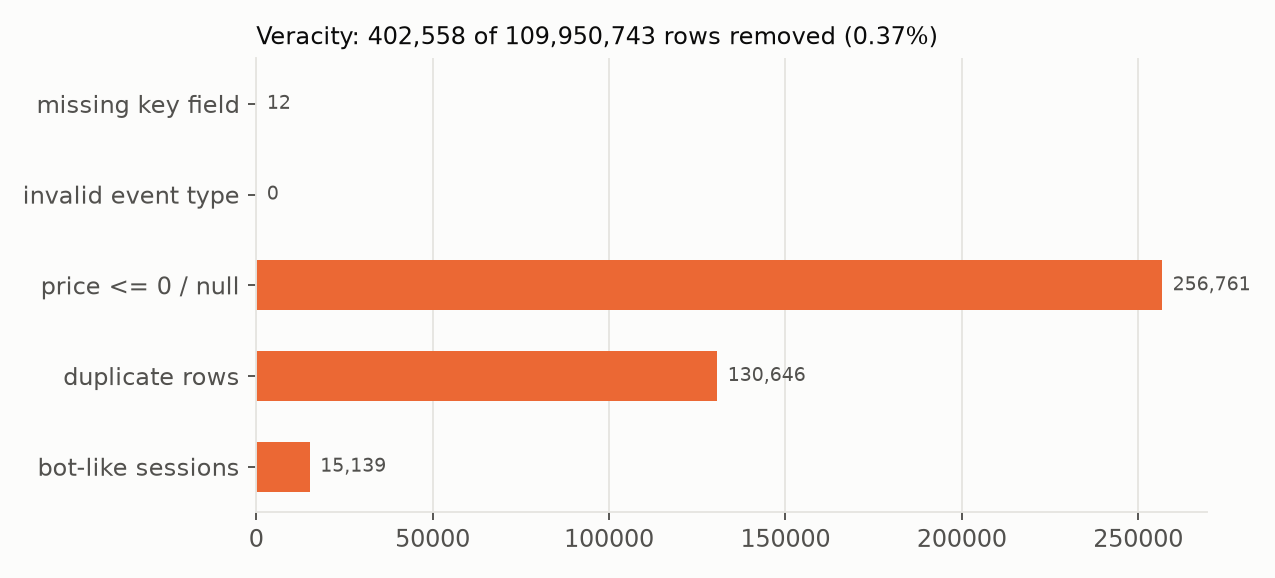
\includegraphics[width=\linewidth]{veracity.png}\\[3pt]
  \shot{\linewidth}{2.2cm}{1}  \end{columns}
\end{frame}

% ---------- 4 ----------
\begin{frame}{System architecture}
  \centering
  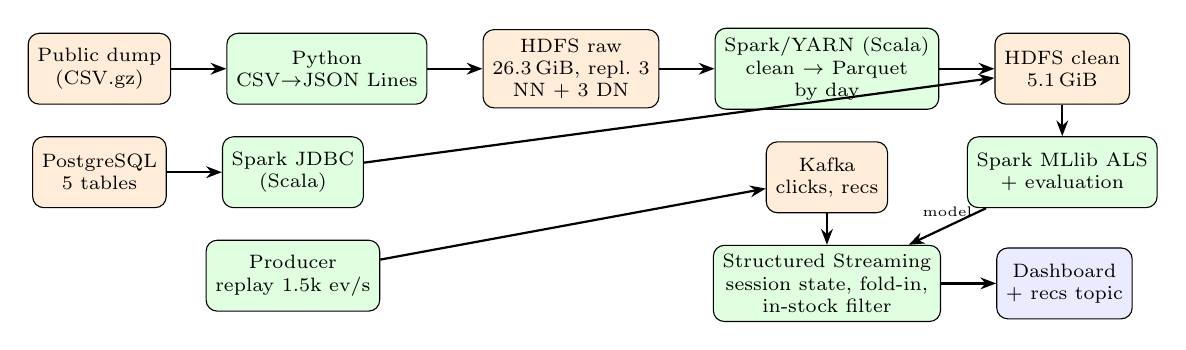
\begin{tikzpicture}[node distance=4mm and 7mm]
    \node[store] (csv) {Public dump\\(CSV.gz)};
    \node[proc,right=of csv] (conv) {Python\\CSV$\to$JSON Lines};
    \node[store,right=of conv] (hdfs) {HDFS raw\\26.3\,GiB, repl.\ 3\\NN + 3 DN};
    \node[store,below=of csv] (pg) {PostgreSQL\\5 tables};
    \node[proc,right=of pg] (jdbc) {Spark JDBC\\(Scala)};
    \node[proc,right=of hdfs] (etl) {Spark/YARN (Scala)\\clean $\to$ Parquet\\by day};
    \node[store,right=of etl] (clean) {HDFS clean\\5.1\,GiB};
    \node[proc,below=of clean] (als) {Spark MLlib ALS\\+ evaluation};
    \node[store,below=of etl] (kafka) {Kafka\\clicks, recs};
    \node[proc,below=of jdbc] (prod) {Producer\\replay 1.5k ev/s};
    \node[proc,below=of kafka] (ss) {Structured Streaming\\session state, fold-in,\\in-stock filter};
    \node[box,right=of ss] (dash) {Dashboard\\+ recs topic};
    \draw[arr] (csv)--(conv); \draw[arr] (conv)--(hdfs); \draw[arr] (pg)--(jdbc); \draw[arr] (jdbc)--(clean);
    \draw[arr] (hdfs)--(etl); \draw[arr] (etl)--(clean); \draw[arr] (clean)--(als);
    \draw[arr] (prod)--(kafka); \draw[arr] (kafka)--(ss); \draw[arr] (als) -- node[above,font=\tiny]{model} (ss);
    \draw[arr] (ss)--(dash);
  \end{tikzpicture}\\[2pt]
  \scriptsize Docker on WSL2 (12\,GB): 1 NameNode, 3 DataNodes, ResourceManager, 1 NodeManager, HistoryServer, Kafka (KRaft), PostgreSQL, Spark 3.5.1 client.
\end{frame}

% ---------- 5 ----------
\begin{frame}{Spark workflow: DataFrame operations, DAG, partitioning, caching}
  \begin{columns}[T]
  \column{0.30\textwidth}
  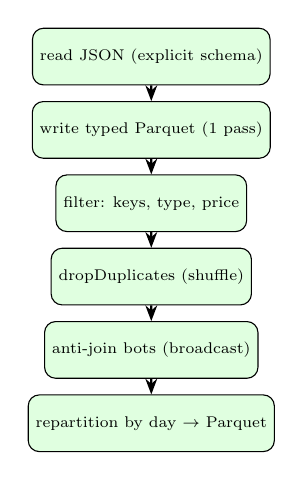
\begin{tikzpicture}[node distance=2.5mm,scale=0.8,transform shape]
    \node[proc] (a) {read JSON (explicit schema)};
    \node[proc,below=of a] (b) {write typed Parquet (1 pass)};
    \node[proc,below=of b] (c) {filter: keys, type, price};
    \node[proc,below=of c] (d) {dropDuplicates (shuffle)};
    \node[proc,below=of d] (e) {anti-join bots (broadcast)};
    \node[proc,below=of e] (f) {repartition by day $\to$ Parquet};
    \foreach \x/\y in {a/b,b/c,c/d,d/e,e/f} \draw[arr] (\x)--(\y);
  \end{tikzpicture}
  \column{0.36\textwidth}
  \footnotesize
  \textbf{Choices (measured, 1 run each)}
  \begin{itemize}\scriptsize
    \item Parquet scan 1.1\,s vs JSON 8.8\,s
    \item 8 files read 0.2\,s vs 500 small files 1.5\,s
    \item Broadcast join 1.1\,s vs sort-merge 3.1\,s
    \item Partition pruning 0.11\,s vs 1.84\,s
    \item 24 shuffle partitions 3.1\,s; 400: 12.6\,s
    \item Cache: 14.8\,s with fill vs 5.6\,s uncached; wins only on re-use (3.9\,s)
  \end{itemize}
  \column{0.32\textwidth}
  \shot{\linewidth}{5.6cm}{2}\\[-1pt]{\tiny Spark UI plan (week of clean events, broadcast join): only 7 day-partitions read}
  \end{columns}
\end{frame}

% ---------- 6 ----------
\begin{frame}[fragile]{Scala implementation: key code and project structure}
  \begin{columns}[T]
  \column{0.56\textwidth}
\begin{lstlisting}[basicstyle=\ttfamily\tiny]
// FoldIn.scala: re-solve a session vector, no retraining
def sessionVector(f: ItemFactors, session: Seq[(Long, Double)],
    lambda: Double, alpha: Double): Option[Array[Double]] = {
  val known = session.flatMap { case (id, r) =>
    f.index.get(id).map(_ -> r) }
  if (known.isEmpty) None else {
    val a = Array.tabulate(f.rank, f.rank)((i, j) =>
      f.gram(i)(j) + (if (i == j) lambda * known.size else 0.0))
    val b = new Array[Double](f.rank)
    known.foreach { case (idx, w) => /* add (c-1) y y^T and c y */ }
    Some(solveSpd(a, b))            // Cholesky solve
  }
}
// pattern matching on event kinds (sealed trait)
def kindOf(t: String): Option[EventKind] = t match {
  case "view"     => Some(View)
  case "cart"     => Some(Cart)
  case "purchase" => Some(Purchase)
  case _          => None
}
\end{lstlisting}
  \scriptsize\textbf{src/scala/.../bda/:} Common, Preprocess, IngestRelational, FoldIn, TrainEval, StreamingJob, TuningBench. Python: converter, producer, charts, dashboard. MapReduce: Streaming job (counts match Spark).
  \column{0.42\textwidth}
  \shot{\linewidth}{6.2cm}{3}\par\vspace{1pt}\tiny VS Code: project tree and FoldIn.scala
  \end{columns}
\end{frame}

% ---------- 7 ----------
\begin{frame}{Spark ML pipeline: features, algorithms, tuning}
  \begin{columns}[T]
  \column{0.5\textwidth}
  \footnotesize
  \textbf{Features:} implicit strength view=1, cart=3, purchase=5 summed per (user,item); catalogue = 45{,}863 items with $\ge$30 training users; 25\% user sample, 10.96\,M training pairs.\\[3pt]
  \textbf{Algorithms:} popularity; MLlib implicit ALS (batch); \textbf{ALS + fold-in}; item co-occurrence; hybrid (reciprocal-rank fusion).\\[3pt]
  \textbf{Protocol:} strict temporal split (train to Nov 20, test Nov 21--30); 159{,}629 next-item cases; HR/MRR/NDCG@20.\\[3pt]
  \textbf{Tuning on a validation window} (never the test window): rank 16/32/64/128, alpha 20/40, reg 0.05/0.2. Rank 128: NDCG 0.228 vs 0.205 (rank 64) but 4.5$\times$ training time (304\,s vs 67\,s) $\to$ final rank 64.
  \column{0.48\textwidth}
  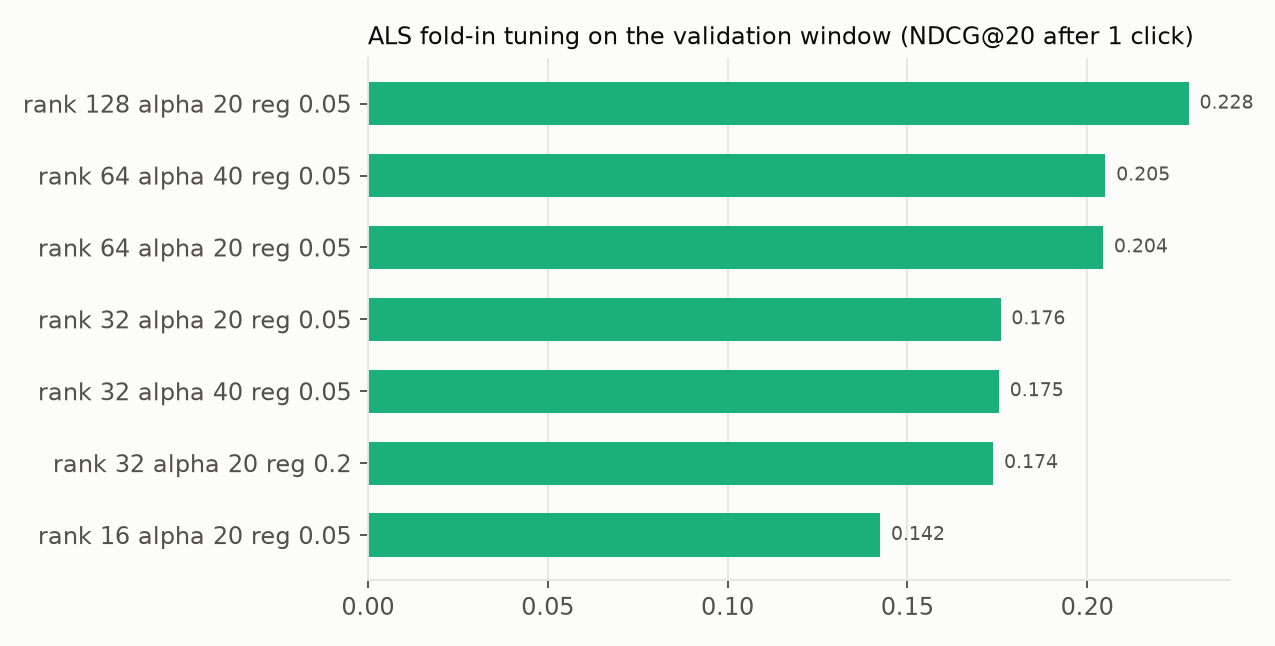
\includegraphics[width=\linewidth]{als_grid.png}\\[3pt]
  \shot{\linewidth}{1.6cm}{4}  \end{columns}
\end{frame}

% ---------- 8 ----------
\begin{frame}{Results: metrics, model comparison, business insight}
  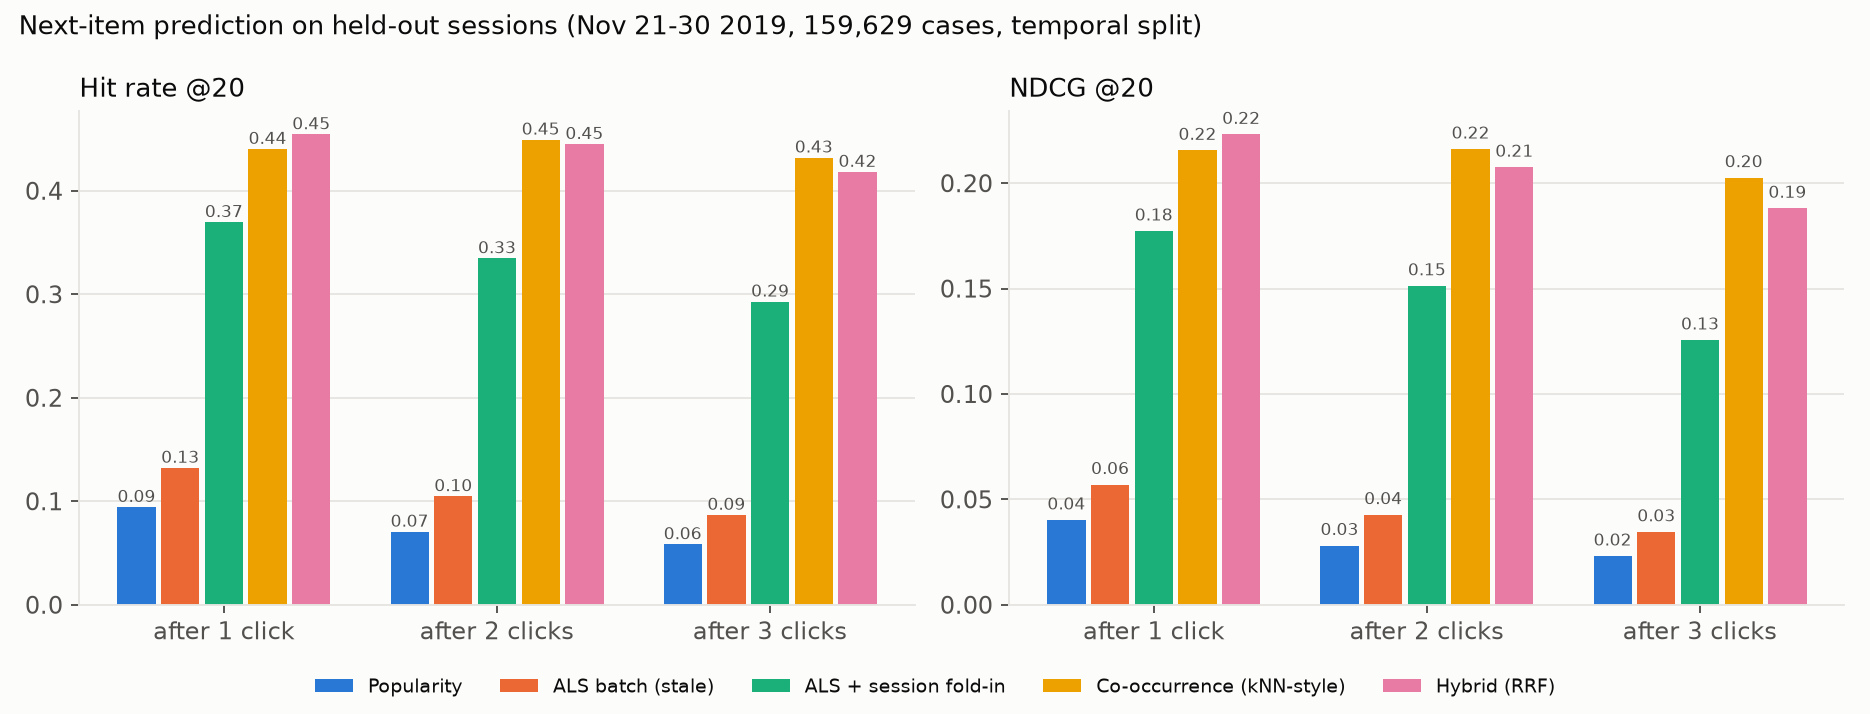
\includegraphics[width=0.62\linewidth]{eval_methods.png}\hfill
  \begin{minipage}[t]{0.35\linewidth}\scriptsize
    \textbf{After 1 click (HR@20 / NDCG@20)}\\
    Popularity 0.094 / 0.040\\
    Batch ALS (stale) 0.132 / 0.057\\
    \textbf{ALS + fold-in} 0.370 / 0.177\\
    Co-occurrence 0.440 / 0.216\\
    Hybrid 0.454 / 0.223\\[3pt]
    \textbf{Insight:} freshness matters (fold-in $\approx$2.8$\times$ stale ALS), but a simple co-occurrence list is the strongest single model -- consistent with the base paper.\\[3pt]
    \textbf{Streaming:} 44{,}613 recs from 135\,k events; latency p50 8.5\,s, p99 20.1\,s.\\[3pt]
  \end{minipage}
\end{frame}

% ---------- 9 ----------
\begin{frame}{Challenges, limitations, conclusion, future work}
  \begin{columns}[T]
  \column{0.5\textwidth}
  \footnotesize\textbf{Challenges and limitations}
  \begin{itemize}\scriptsize
    \item 16\,GB laptop: WSL2 12\,GB, 1.25\,GB executors, 1 NodeManager
    \item 25\% user sample, single runs, no significance tests
    \item Catalogue limited to 45.9\,k popular items
    \item Users and inventory are synthetic; velocity is simulated replay
    \item Latency is seconds, not milliseconds
    \item No neural / full SKNN baselines; fold-in weakens with longer sessions (cause not investigated)
    \item 3 DataNodes share one disk (no real fault tolerance)
  \end{itemize}
  \column{0.48\textwidth}
  \footnotesize\textbf{Conclusion}\\
  A reproducible Hadoop/Spark/Kafka platform processes 110\,M events on a laptop. Fold-in makes ALS fresh at ms cost; co-occurrence still wins; hybrid helps at the first click.\\[4pt]
  \textbf{Future work}
  \begin{itemize}\scriptsize
    \item Prequential evaluation with significance tests
    \item GRU4Rec / SKNN baselines (Kaggle GPU)
    \item Multi-broker Kafka, Kafka Connect to HDFS
    \item Online A/B test
  \end{itemize}
  \end{columns}
\end{frame}

% ---------- 10 ----------
\begin{frame}[allowframebreaks]{References and GitHub link}
  \scriptsize
  \textbf{GitHub:} \url{https://github.com/kirupashankarchockkanathan/Clickstream-Recommender}\\[3pt]
  \begin{thebibliography}{9}
  \bibitem{r1} M.~Ludewig, N.~Mauro, S.~Latifi, D.~Jannach, ``Empirical analysis of session-based recommendation algorithms,'' \emph{User Model.\ User-Adap.\ Inter.}, vol.~31, pp.~149--181, 2021, doi:10.1007/s11257-020-09277-1.
  \bibitem{r2} S.~Wang, L.~Cao, Y.~Wang, Q.~Z.~Sheng, M.~A.~Orgun, D.~Lian, ``A survey on session-based recommender systems,'' \emph{ACM Comput.\ Surv.}, vol.~54, no.~7, art.~154, 2021, doi:10.1145/3465401.
  \bibitem{r3} M.~Jakomin, Z.~Bosni\'c, T.~Curk, ``Simultaneous incremental matrix factorization for streaming recommender systems,'' \emph{Expert Syst.\ Appl.}, vol.~160, art.~113685, 2020, doi:10.1016/j.eswa.2020.113685.
  \bibitem{r4} J.~Vinagre, A.~M.~Jorge, C.~Rocha, J.~Gama, ``Statistically robust evaluation of stream-based recommender systems,'' \emph{IEEE Trans.\ Knowl.\ Data Eng.}, vol.~33, no.~7, 2021, doi:10.1109/TKDE.2019.2960216.
  \bibitem{r5} Y.~Ji, A.~Sun, J.~Zhang, C.~Li, ``A critical study on data leakage in recommender system offline evaluation,'' \emph{ACM Trans.\ Inf.\ Syst.}, vol.~41, no.~3, art.~75, 2023, doi:10.1145/3569930.
  \bibitem{r6} T.~P.~Raptis, A.~Passarella, ``A survey on networked data streaming with Apache Kafka,'' \emph{IEEE Access}, 2023, doi:10.1109/ACCESS.2023.3303810.
  \bibitem{r7} M.~Zaharia et al., ``Apache Spark: A unified engine for big data processing,'' \emph{Commun.\ ACM}, vol.~59, pp.~56--65, 2016, doi:10.1145/2934664.
  \bibitem{r8} M.~Kechinov, ``eCommerce behavior data from multi-category store,'' REES46 Open CDP, Kaggle.
  \end{thebibliography}
\end{frame}

% ---------- appendix: demo screenshots ----------
\appendix
\begin{frame}{Backup: HDFS evidence (replication 3, three live DataNodes)}
  \begin{columns}[T]
  \column{0.33\textwidth}\shot{\linewidth}{3.2cm}{6}\\{\tiny DataNodes tab: 3 in service}
  \column{0.33\textwidth}\shot{\linewidth}{3.2cm}{7}\\{\tiny fsck: HEALTHY, avg.\ replication 3.0}
  \column{0.33\textwidth}\shot{\linewidth}{3.2cm}{8}\\{\tiny clean data, one folder per day}
  \end{columns}
\end{frame}

\begin{frame}{Backup: streaming demo evidence}
  \begin{columns}[T]
  \column{0.5\textwidth}\shot{\linewidth}{3.4cm}{10}\\{\tiny YARN: M4-streaming application RUNNING}\\[3pt]\shot{\linewidth}{3.0cm}{9}\\{\tiny messages on Kafka topic recs (session, clicks, 10 recommended items)}
  \column{0.48\textwidth}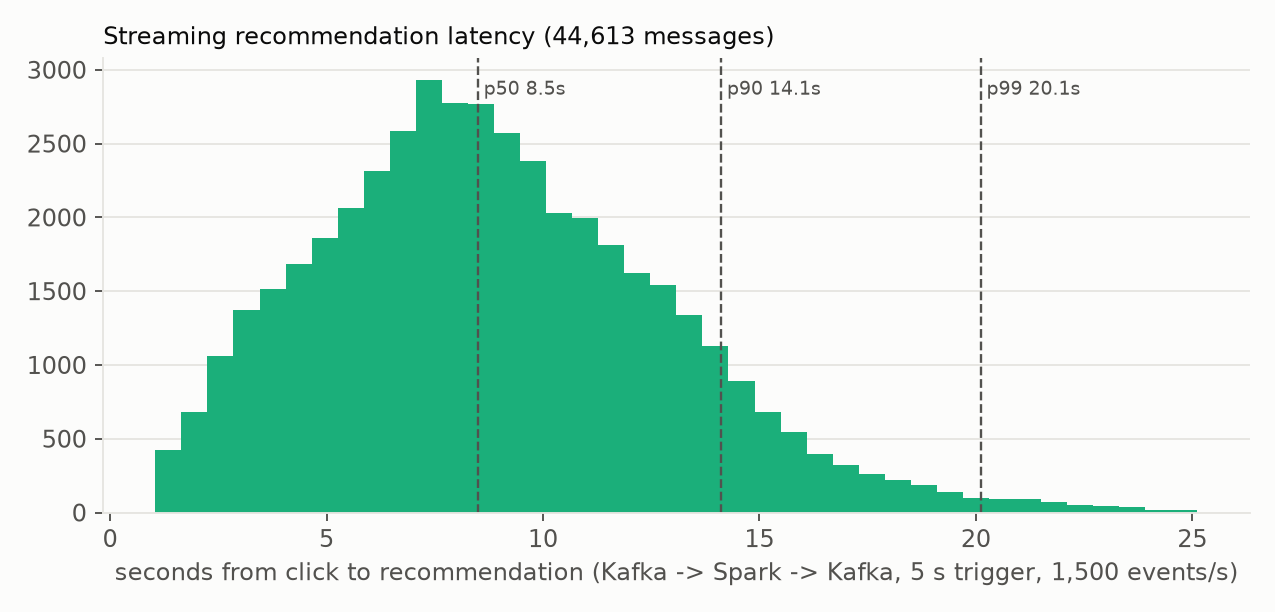
\includegraphics[width=\linewidth]{stream_latency.png}
  \end{columns}
\end{frame}

\begin{frame}{Backup: dashboard and tuning results}
  \begin{columns}[T]
  \column{0.46\textwidth}\shot{\linewidth}{5.4cm}{5}\\{\tiny Streamlit dashboard, Accuracy tab (grouped bars)}
  \column{0.52\textwidth}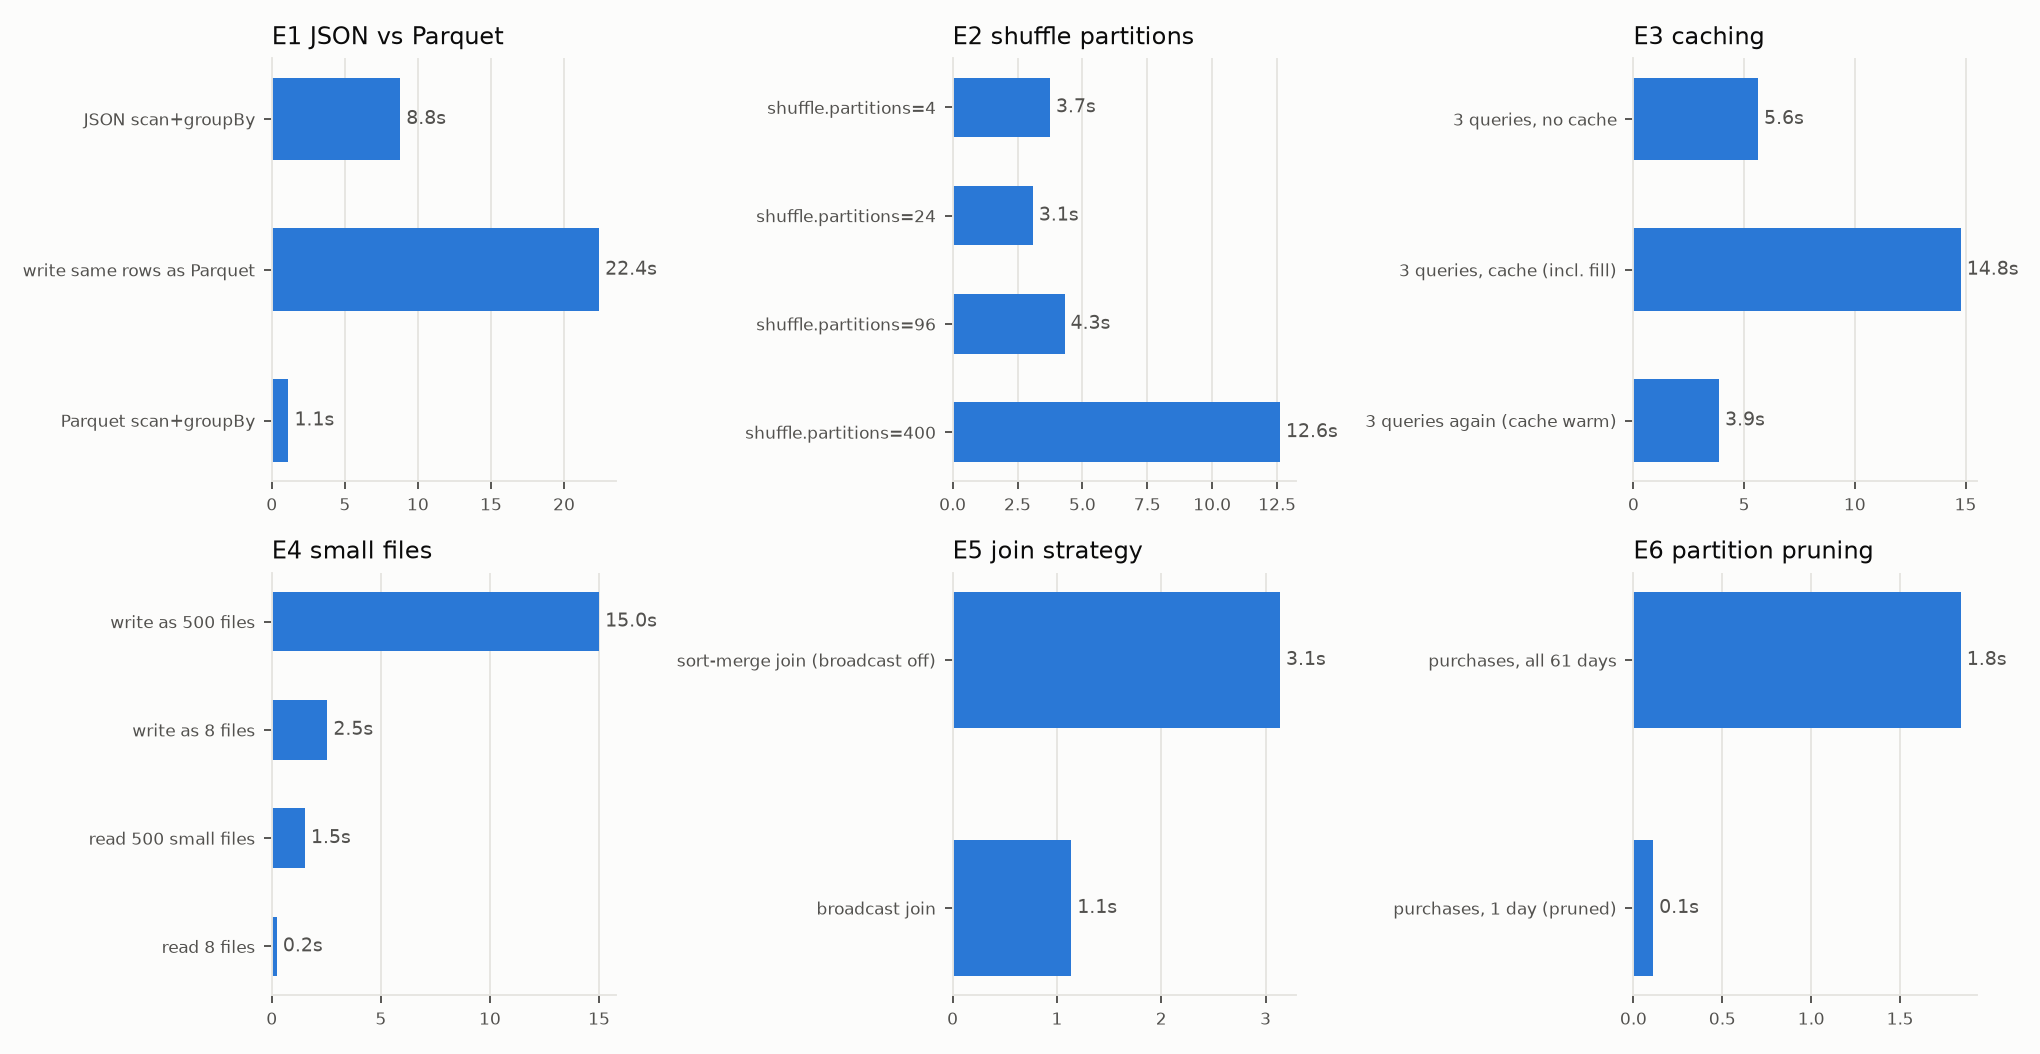
\includegraphics[width=\linewidth]{tuning.png}
  \end{columns}
\end{frame}

\end{document}
